\documentclass[margin=0.1in]{standalone}
\usepackage{tikz}
\usetikzlibrary{snakes}
\usepackage{stanli}
\begin{document}

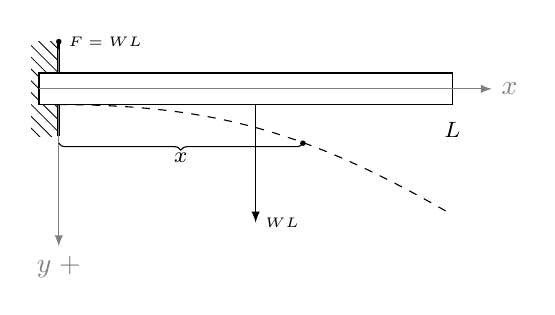
\begin{tikzpicture}[>=latex]
	\point{a}{0}{0}
	\support{3}{a}[-90];
	\draw [gray,->] (0,0.5) --++ (0,-2.5) node [below] {\(y\;+\)};
	\filldraw [fill=white ,semithick] (-0.25,-0.2) rectangle (5,0.2) node [below=5mm] {\footnotesize  \(L\)};
	\draw [gray,->] (-0.25,0) -- (5.5,0) node [right] {\(x\)};
	\draw [dashed] (0,-0.2) to [out=0 , in=180-30] (5,-1.6);
	\fill (0,0.6) circle (1pt) node [right] {\tiny  \(F=WL\)};
	\coordinate (A) at (3.1,-0.69);
	\fill (A) circle (1pt);
	\draw [snake = brace, mirror snake] (0,-0.69) to node [below] {\footnotesize \(x\)} (A);
	\draw [->] (2.5,-0.2) --++ (0,-1.5) node [right] {\tiny \(WL\)};
\end{tikzpicture}

\end{document}
